% Created 2023-12-03 Sun 17:34
% Intended LaTeX compiler: pdflatex
\documentclass[12pt, a4paper]{article}
\usepackage[utf8]{inputenc}
\usepackage[T1]{fontenc}
\usepackage{graphicx}
\usepackage{longtable}
\usepackage{wrapfig}
\usepackage{rotating}
\usepackage[normalem]{ulem}
\usepackage{amsmath}
\usepackage{amssymb}
\usepackage{capt-of}
\usepackage{hyperref}
\usepackage{placeins}
\usepackage{gensymb}
\usepackage[letterpaper]{geometry}
\geometry{top=1.0in, bottom=1.0in, left=1.0in, right=1.0in}
\usepackage{rotating}
\usepackage{graphicx}
\usepackage{pgfplots}
\usepackage{filecontents}
\usepackage{tikz}
\usepackage{fancyhdr}
\usepackage{enumitem}
\pagestyle{fancy}
\lhead{}
\chead{}
\rhead{Johnson \thepage}
\lfoot{}
\cfoot{}
\rfoot{}
\renewcommand{\headrulewidth}{0pt}
\renewcommand{\footrulewidth}{0pt}
\setlength\headsep{0.333in}
\newcommand{\bibent}{\noindent \hangindent 40pt}
\newenvironment{workscited}{\newpage \begin{center} Works Cited \end{center}}{\newpage }
\graphicspath{ {./attachments/} }
\author{Christian}
\date{\today}
\title{}
\hypersetup{
 pdfauthor={Christian},
 pdftitle={},
 pdfkeywords={},
 pdfsubject={},
 pdfcreator={Emacs 28.2.50 (Org mode 9.7-pre)}, 
 pdflang={English}}
\begin{document}

\begin{document}
\begin{flushleft}
Christian Johnson\\
\vspace{2mm}Dr. Paul Crilly\\
\vspace{2mm}Antennas and Propogation\\
\vspace{2mm}December 03 2023\\
\vspace{4mm}\begin{center}
Lab 9 Report
\end{center}
\vspace{1mm}\setlength{\parindent}{0.5in}
\begin{abstract}
In this Antennas and Propagation Laboratory Exercise, our group utilized Yagi antennas in conjunction with the Agilent 9912A Field Fox Analyzer to locate a hidden transmitter operating at 146.5 MHz on our campus. Employing radio direction finding techniques, we aimed to efficiently determine the transmitter's location. The report provides a concise overview of our methodology, results, and insights.
\end{abstract}
\section*{Introduction}
\label{sec:org6454ee2}
Radio direction finding is a critical aspect of wireless communication, allowing the determination of the location of a radio frequency source. In our Antennas and Propagation Laboratory Exercise, we delved into the practical application of this concept using Yagi antennas. At very high frequencies (VHF), the Yagi antenna's high front-to-back and front-to-side ratio makes it an invaluable tool for locating radio frequency (RF) sources. The primary objective of this exercise was to employ our newly constructed Yagi antennas in conjunction with the Agilent 9912A Field Fox Analyzer to locate a hidden transmitter operating at 146.5 MHz on our campus.
\section*{Procedure}
\label{sec:org5a1f818}
Our methodology involved setting up the N9912A to receive signals from 144 to 148 MHz, activating the averaging option, and configuring the bandwidth to minimize the impact of minor signal variations on our ability to determine the bearing of the hidden transmitter. Each group, comprising individuals who had participated in the construction of the Yagi antennas, was tasked with locating a hidden "fox" transmitter, which emitted an intermittent 146.5 MHz beacon. A member from a different group concealed the transmitter in a location at least 1000 feet away, ensuring a challenging search. The importance of differentiating the fox's signal from other RF sources, including multipath signals, signals from other foxes, and users on the 144 MHz band, was emphasized.
\section*{Results and Conclusions}
\label{sec:org7c87850}
Our findings revealed the effectiveness of the Yagi antennas in locating the hidden transmitter. The time taken to pinpoint the fox was just under 5 minutes, showcasing the efficiency of our radio direction finding approach. However, challenges emerged in the form of multipath signals and interference from other foxes or users on the 144 MHz band. These incidents prompted us to refine our search process and try a second time, resulting in a marginally reduced time and contributing to an enhanced skill set in locating RF sources. Insights gained from the exercise were documented, highlighting the importance of factors such as front-to-back and front-to-side ratios in Yagi antennas.

\newpage
\begin{center}
Appendices
\end{center}
\begin{figure}[htb]
\centering
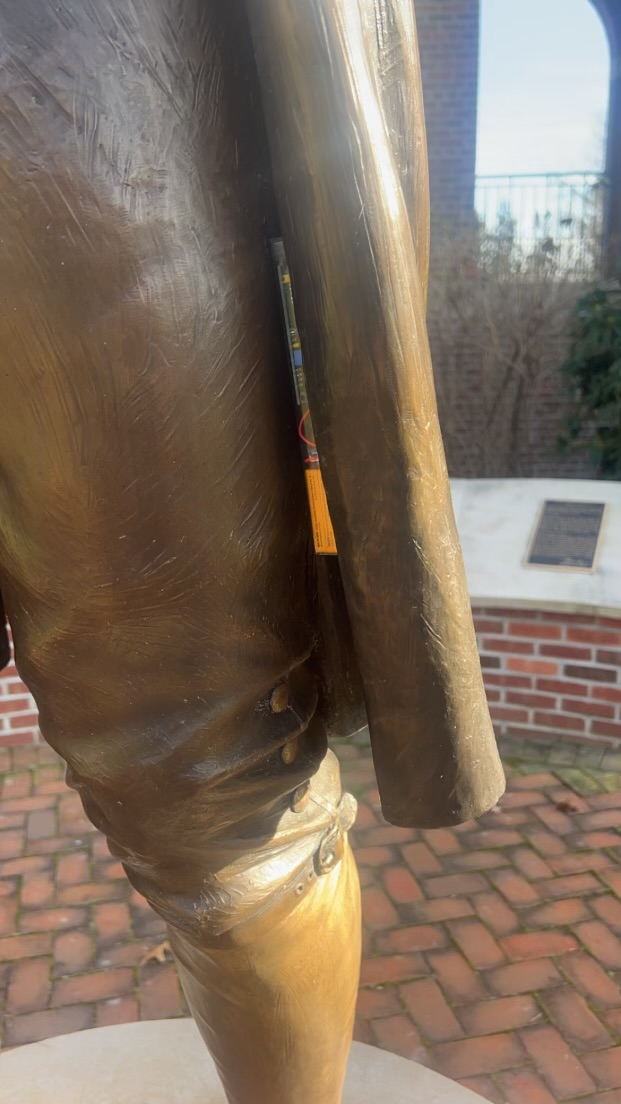
\includegraphics[width=0.4\textwidth]{Fox.jpg}
\caption{Transmitter Hiding Location}
\end{figure}
\begin{figure}[htb]
\centering
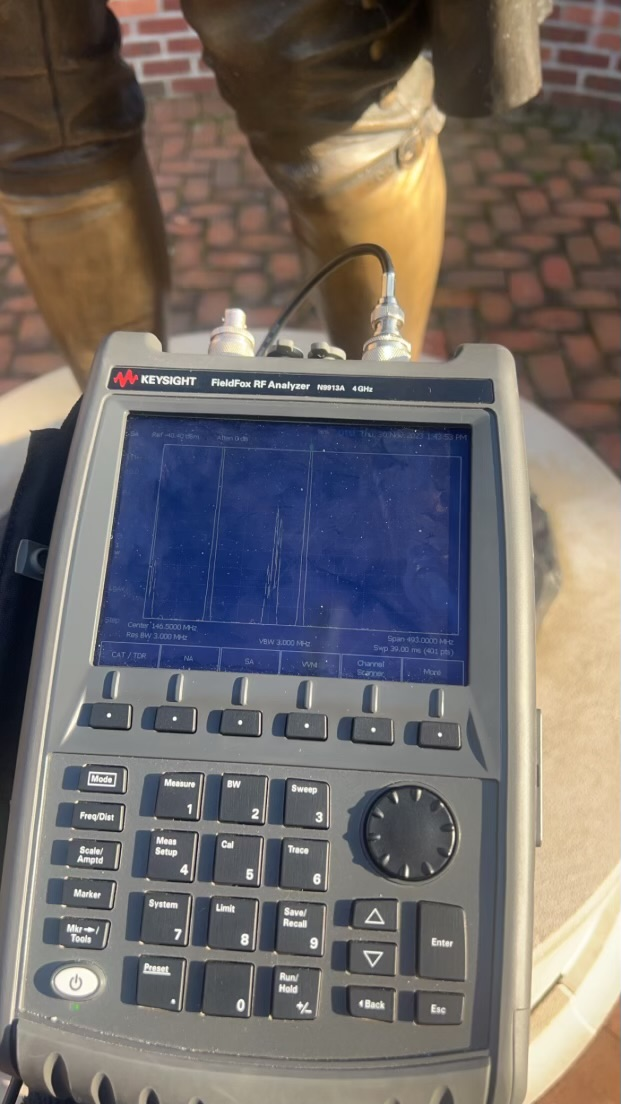
\includegraphics[width=0.7\textwidth]{FieldFox.jpg}
\caption{Field Fox Graph}
\end{figure}
\newpage

\end{document}
\end{document}